In this chapter, we will motivate the problem tackled by this thesis and highlight the challenges involved. We will then present necessary background to understand the rest of the thesis by formally laying out the problems of path planning and trajectory prediction. We finish the chapter by describing the organization of the thesis. 

\section{Planning and Dynamics}
\label{sec:intro-motivation}

Navigation is an essential task for the autonomous mobile robot. The task not only involves how the robot can move on its own, but also how to achieve various goals and objectives. Specifically, the robot has to achieve its goals in the presence of hard constraints such as dynamic feasibility, collision avoidance, and soft constraints such as social compliance. These problems involve finding trajectories in the workspace from a start configuration to a goal configuration that satisfy the aforementioned constraints. \textit{Path Planning} is the problem of finding such a trajectory. The path planning approach depends on two important properties of the planner: The agent needs to have an accurate model of the dynamics of the environment or state of the world around it, and it needs to have a model of how its actions affect the world state. For mobile robots, this is significantly challenging as they have to rely on perception to create a model of the world state. In the absence of an accurate long-horizon models and limited perception, mobile robots were traditionally relegated to use reactive methods or one-step planning algorithms, \cite{fox1997dynamic,brock1999high}. These reactive methods map the observed state of the world at the current time-step to an action for the robot to execute. Employing an accurate model of the environment, the mobile robot can instead plan its actions ahead, to achieve more efficient (in some cases, more social) behavior. However, the major challenge in achieving this objective is modeling the state of the environment, which can be dynamic.

Dynamics is an important aspect of mobile robot navigation in partially known or completely unknown environments. Robot dynamics are the kinematic and dynamic constraints that need to be considered while planning the path of the robot. Most modern planning algorithms consider these kinodynamic constraints to come up with feasible trajectories for the robot to execute. The other kind of dynamics in navigation is, dynamics of the world or environment. An environment where other agents or obstacles move is said to be dynamic. A major challenge in navigation is to come up with an accurate model for their motion, so that it can be accounted while planning the path of the robot. Such a model needs to result in accurate long-term predictions of the trajectories of other agents in the environment. More often than not, dynamics of the environment are not readily predictable and need to be supplemented by sensory information. Given sensory information regarding the past behavior of the agents, the model needs to predict their future behavior.

In this thesis, we focus on the problems of planning and modeling dynamics. More specifically, the first part of the thesis deals with  path planning in dynamic environments and the latter half deals with human trajectory prediction in dense crowds. We present novel solutions and take a small step towards making the goal of autonomous mobile robot navigation more realizable.

\section{Motivation}
\label{sec:intro-motiv-chall}

We envision mobile robots to coexist with humans in unscripted environments and accomplish various kinds of tasks. Existing works towards this goal started out in the 1990s with RHINO, \cite{thrun99}, and MINERVA, \cite{Thrun2000ProbabilisticAA}, both designed as interactive museum tour guide robots that will move among humans in museums. These works made extensive use of path planning, localization and mapping methods that were developed around the same time. These works pioneered the field of service robots inciting a period of exciting research in the area of robot navigation in human crowds. Chapter \ref{chap:survey} discusses several of the subsequent works.

Despite the decades of research towards this goal, there are several fundamental problems that remain unsolved. Traditional algorithms for navigation in dynamic environments tend to make strong assumptions about the environment and its own motion model, in order to efficiently plan paths quickly \cite{lavalle2006planning, latombe2012robot}. These planning algorithms don't extend readily to unscripted environments where the agent is highly uncertain about the dynamics of the environment. Most of the works towards modeling dynamics of an unknown environment make simplifying reductions such as independence of motion and the number of surrounding agents \cite{choset2005principles}. Situations where the actions of each agent affect that of the other (especially, in the case of human-robot interaction) are not modeled. To make the vision of coexisting robots and humans a reality, there is a great need for efficient planning algorithms in dynamic environments and accurate models for environment dynamics.

\section{Problem Definition}
\label{sec:intro-background}

In this section, we describe the formal problem definitions for the path planning and trajectory prediction problems. Subsequently, we describe how planning can be reduced to inference in a joint prediction model and briefly present the \textit{freezing robot problem}, which was first introduced in \cite{trautman10}.

%\subsection{Notation}
%\label{sec:intro-notation}

%For the rest of this thesis, we will adhere to the following notation:
%\begin{itemize}
%\item $G$ : Graph representing a discretized state-space that is searched
%\item $S$ : Set of discretized states in the search space
%\item $T$ : Set of feasible transitions between any two states in $S$
%\item $c$ : Cost function encoding the cost of each transition in $T$
%\item $X_s$ : Start state (an element of $S$)
%\item $X_g$ : Goal state (an element of $S$)
%\item $\pi(X_i, X_j)$ : A path in $G$ between two states $X_i$ and $X_j$ in $S$ using $T$
%\item $\pi^*(X_i, X_j)$ : Minimum cost path in $G$ between states $X_i$ and $X_j$
%\item $\epsilon$ : Heuristic inflation factor
%\item $\fbold$ : Trajectory as a mapping from discrete time-step $t$ to $(x,y) \in \mathbb{R}^2$ in continuous space
%\item $\zbold$ : Observed locations in $\mathbb{R}^2$ at discrete time-steps
%\item $g$ : Goal location in continuous $\mathbb{R}^2$ space
%\end{itemize}

\subsection{Path Planning Problem}
\label{sec:intro-path-plann-probl}
The general path planning problem for an explicit goal configuration is, given the robot dynamics, its start configuration and the configuration space, to find a path that is collision-free, dynamically feasible to execute and is a solution.


Let $X \subset \mathbb{R}^n$ be the configuration space of the system. Let $X_{obs} \subset X$ be invalid configurations that result in collision with obstacle. The dynamics of the system is specified as a dynamics constraint $g(x, \frac{dx}{dt}, \dots, \frac{d^rx}{dt^r}) \leq 0, x \in X$, where $r$ is the relative degree. Let the trajectory $\xi: [0, 1] \rightarrow X$ be a continuous mapping from time to configuration. The planning problem is to find the shortest dynamically feasible trajectory from start $x_0$ to the goal $x_f$ that is collision free. This is expressed as follows:

\begin{equation}
\begin{aligned}
\label{eq:planning-problem}
& \underset{x(t)}{\text{minimize}} & & \int\limits_0^1 \| \dot{x}(t) \| \mathrm{dt} \\
& \text{subject to} & & x(0) = x_0 \\
&                   & & x(1) = x_f \\
&                   & & g(x, \frac{dx}{dt}, \dots, \frac{d^rx}{dt^r}) \leq 0 \\
&				    & & x(t) \in X \setminus X_{obs}, t \in [0,1] \\
\end{aligned}
\end{equation}

The above optimization problem seeks to find the shortest trajectory between the start and goal configuration. In the presence of a cost function $c(x_i, x_j)$ that encodes the cost of transition from $x_i$ to $x_j$, the objective of the optimization can be changed appropriately.

\subsection{Trajectory Prediction Problem}
\label{sec:intro-traj-pred-probl}

Trajectory prediction in a dynamic environment entails predicting the future trajectories of all dynamic agents in the environment until a fixed horizon. As argued before, this problem is challenging as we need to model the world dynamics to obtain accurate predictions.

Given a dynamic environment with agents indexed by the set $\{1, 2, \cdots, N\}$, where $N$ is the number of agents in the environment. The trajectory of agent $i$ is given by $\fbold^{(i)} = (f_1^{(i)}, f_2^{(i)}, \cdots, f_T^{(i)})$ where $T$ is the length of trajectory, and $f_t^{(i)}$ represents the location of agent $i$ at time $t$. We also assume that we have access to their past observed locations given by $\zbold$, where $\zbold^{(i)} = (z_1^{(i)}, z_2^{(i)}, \cdots, z_t^{(i)})$ are the observed locations of agent $i$ until time $t$. \\



The trajectory prediction problem is to model the following joint distribution
\begin{equation}
  \label{eq:traj-prediction-problem}
  P(\fbold^{(1)}, \fbold^{(2)}, \cdots, \fbold^{(N)} | \zbold^{(1)}, \zbold^{(2)}, \cdots, \zbold^{(N)})
\end{equation}
i.e., given their observed locations $\zbold^{(1)}, \zbold^{(2)}, \cdots, \zbold^{(N)}$, we want to estimate the distribution over their trajectories until some future time $T$. Note that such joint modeling accounts for dependencies between trajectories of different agents which, as we show later, is paramount for accurate predictions.

\subsection{The Freezing Robot Problem}
\label{sec:intro-plann-as-infer}
%\label{sec:intro-freez-robot-probl}

The freezing robot problem, first introduced in \cite{trautman10}, highlights the deficiencies of existing predictive models that force the robot to come to a complete stop (or freeze). \cite{trautman10} shows that even under \textit{perfect individual prediction} for all agents in the environment, the freezing robot problem can occur for certain configurations. Figure \ref{fig:intro-freeze} shows a common scenario in human crowds, where people walking shoulder-to-shoulder towards the robot, forces it to go around the crowd or in the worst case, stop completely.
% As in \cite{trautman10}, this happens as most navigation approaches ignore mathematical models of cooperation between humans and the robot.
As shown in \cite{trautman10}, this happens as most existing navigation approaches ignore implicit cooperation between humans and the robot. 

\begin{figure}
  \centering
  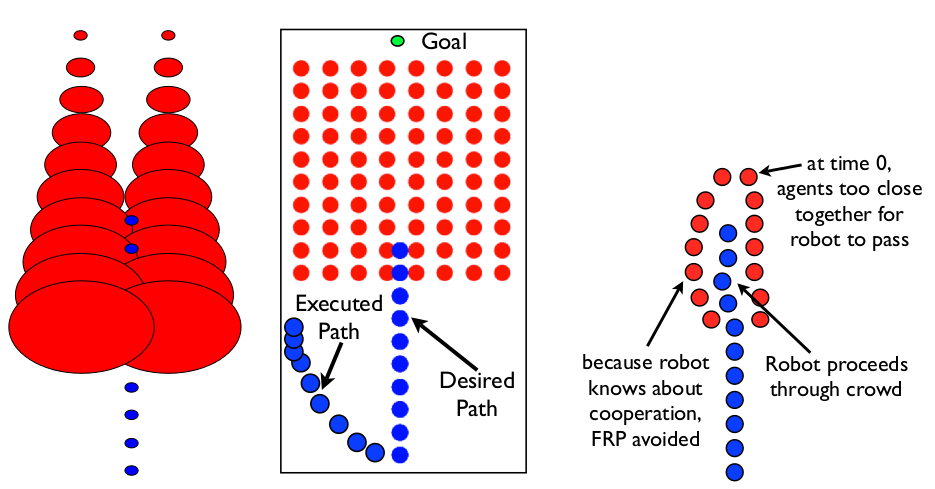
\includegraphics[width=\linewidth]{Figures/frp.png}
  \caption{Example of Freezing Robot Problem, \cite{trautman10}}
  \label{fig:intro-freeze}
\end{figure}

The key insight, which we will follow in this thesis, is that agents engage in \textit{joint collision avoidance}, i.e. they adapt their trajectories to make room for other agents to navigate. The joint collision avoidance criteria has been shown to improve tracking of humans in dense crowds, \cite{pellegrini09, trautman10, trautman13, trautman15}.

The approach, suggested in \cite{trautman10}, to solve the freezing robot problem is to move away from individual agent prediction and model the joint distribution of trajectories, as shown in equation \ref{eq:traj-prediction-problem}. In addition to joint modeling, we need to model the robot as one of the agent so that we also include interactions between the robot and other agents. In other words, the prediction algorithm should model
\begin{equation}
  \label{eq:freeze}
  P(\fbold^{(R)}, \fbold^{(1)}, \fbold^{(2)}, \cdots, \fbold^{(N)} | \zbold^{(1)}, \zbold^{(2)}, \cdots, \zbold^{(N)})
\end{equation}
where $\fbold^{(R)}$ is the robot's trajectory. Note that this distribution encodes the idea of \textit{cooperative planning} as it captures interactions among agents and the robot.

An interesting outcome from this modeling is that planning the robot's trajectory reduces to inference in this joint model, i.e. inferring what the robot should do given the actions of other agents.
\begin{equation}
  \label{eq:planning-reduced-to-inference}
  (\fbold^{(R)}, \fbold^{(1)}, \cdots, \fbold^{(N)})^* = \argmax_{(\fbold^{(R)}, \fbold^{(1)}, \cdots, \fbold^{(N)})} P(\fbold^{(R)}, \fbold^{(1)}, \cdots, \fbold^{(N)} | \zbold^{(1)}, \cdots, \zbold^{(N)})
\end{equation}

As we will see in Chapter \ref{chap:oigp}, this results in ``human-like'' behavior for the robot when modeling crowds, as we model the robot as one of the humans. 


\section{Thesis Organization}
\label{sec:intro-thesis-organization}

The remainder of this thesis is organized as follows: Chapter \ref{chap:survey} presents a brief survey of past works in the domain of robot navigation in human crowds. We also list out several works in the domain of human tracking in crowds and video surveillance. Chapter \ref{chap:ppad} presents our novel approach to solving the problem of efficient path planning in dynamic environments when an accurate model of the world dynamics is known. We propose a heuristic-based graph search algorithm that results in safe and feasible paths for the robot in short planning times. Additionally, we present theoretical guarantees on the optimality of the resulting path and completeness of the planning algorithm. The task of obtaining an accurate model of the world dynamics (specifically, crowd dynamics) is tackled in Chapter \ref{chap:oigp} where we propose a novel statistical modeling approach that couples predictions for multiple agents through occupancy grids. The proposed model is learned from real world trajectory and can be used to predict future trajectories of dynamic agents in an environment. Finally, Chapter \ref{chap:conclusion} summarizes the contributions of this thesis and provides directions for future research in this area.

%%% Local Variables:
%%% mode: latex
%%% TeX-master: "thesis"
%%% End:
